%! TEX root = /home/hsartoris/sproj/writeup/main.tex
\graphicspath{{resources/}}

\chapter{Background}

\section{Biological Neural Networks}
\label{sec:bioNN}
A biological neural network in the sense we will use it here is a collection of 
neurons, the connections between which enable cognition. Neurons themselves 
consist of a cell body, from which emerge axons and dendrites. Axons extend from 
the neuron body to meet the dendrites emerging from another neuron, and this 
forms a connection that, in terms of electrical terms, is one-way.\footnote{This 
needs a citation.} Neurons may connect to and receive connections from many 
other neurons\footnote{again citation}, and the axons can be so long as to 
render physical adjacency of neurons in a network irrelevant in terms of 
connection probability.\footnote{cite again}

\subsection{Neuron Behavior}
Neurons generally sit at a resting voltage\footnote{cite}, but upon receiving a 
high enough total input level from incoming connections to exceed a particular 
threshold, they spike, rapidly increasing in voltage and then dropping again.  
This voltage travels down the neuron's axons and in turn provides input to other 
neurons.
\subsection{Extracting Data}
Due to the three-dimensional nature of most brains, the sheer quantity of 
neurons, and their small size, manually mapping out a brain, and in particular 
the actual connections from neuron to neuron, is practically impossible. In 
order to monitor activity within a biological neural network, then, some 
compromises must be made. Several techniques exist for neuron monitoring; on the 
very small scale is the patch clamp technique, in which a pipette is directly 
attached to a single neuron\cite{neher1992patch}, to in-vivo calcium imaging, in 
which a dye is injected into a living brain, leading the neurons to fluoresce 
when spiking\cite{Stosiek7319}. As calcium imaging allows observation of as many 
neurons as can be seen by a camera, we are interested in data that are derived 
from this process.

\begin{wrapfigure}[8]{r}{.25\textwidth}
	\centering
	\vspace{-14pt}
	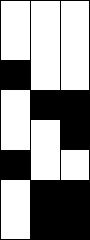
\includegraphics[width=.13\textwidth]{models/3neurEx/fullRun/1_dumb/input.png}
	\captionsetup{width=.85\linewidth}
	\caption{Spike time raster plot}
	\label{fig:rasterplot}
\end{wrapfigure}
Although calcium uptake into neurons during spiking is relatively slow, making 
determination of precise spike time difficult, use of existing deconvolution 
algorithms can facilitate the creation of spike-time raster plots\cite{Xu8025}.  
These plots contain a binary representation of neuron spiking: at each timestep, 
each neuron is either spiking, or not. In \figref{fig:rasterplot}, each column 
corresponds with one neuron, and each row represents a timestep; a filled block 
indicates a spike, and an unfilled block indicates no spike.


\section{Graphs}
In general, we define a graph as a collection of nodes and edges\footnote{This 
is something of an abuse of notation \cite{networksciencebook}}, where nodes 
represent states or components of a system, and edges represent the connections 
between those nodes\cite{networksciencebook}. An example graph can be found in 
\figref{fig:digraph}.

\begin{wrapfigure}[6]{l}{.28\textwidth}
	\centering
	\vspace{-5pt}
	
\begin{tikzpicture}[baseline=(current bounding box.center),->,>=stealth', 
	node distance=5em, semithick]
	\tikzstyle{every state}=[fill=none, draw=black, text=black]

	\node[state] (0) {0};
	\node[state] (1) [right of=0] {1};
	\node[state] (2) [below right of=0] {2};

	\path 	(0) edge node {} (1)
			(0) edge node {} (2)
			(1) edge node {} (2);
\end{tikzpicture}

	\caption{Digraph}
	\label{fig:digraph}
\end{wrapfigure}
\noindent Graphs can be used to describe many systems; for example, social 
groups can be represented in graph form, where people are nodes and friendships 
are edges.  In such a case, the edges in the graph are bidirectional (one 
hopes). In describing other systems, however, edges are often unidirectional.  
Such a graph is called a directed graph, or digraph.\cite{networksciencebook} 
The graphs we consider here will be digraphs in that a biological neural network 
can be thought of as a directed graph: as described in \ref{sec:bioNN}, physical 
adjacency of individual neurons does not necessarily play a role in the 
likelihood of a connection existing. This makes graphs an ideal representation 
for biological neural networks: placement of nodes when visualizing a graph is 
purely arbitrary, with only the nodes and their connections being important.  
Thus we will consider biological neural networks through a graph representation, 
wherein the nodes are neurons and the edges are axons.

\subsection{Graph Structures in Biological Neural Networks}
\label{subsec:motifs}
\begin{wrapfigure}[6]{l}{.3\textwidth}
	\centering
	\vspace{-12pt}
	{\scalebox{.9}{\begin{tikzpicture}[baseline=(current bounding box.center),->,>=stealth', 
	node distance=5em, semithick]
	\tikzstyle{every state}=[fill=none, draw=black, text=black]

	\node[state] (0) {0};
	\node[state] (1) [right of=0] {1};
	\node[state] (2) [below of=0] {2};
	\node[state] (3) [right of=2] {3};

	\path	(0) edge node {} (1)
			(0) edge node {} (2)
			(0) edge node {} (3)
			(1) edge node {} (2)
			(1) edge node {} (3)
			(2) edge node {} (3);

\end{tikzpicture}
}}
	\caption{3-simplex}
	\label{fig:3simplex}
\end{wrapfigure}
Graph analysis of naturally-occurring networks, including neural networks, 
reveals the consistent repetition throughout of small patterns, known as motifs, 
and suggests that network robustness towards perturbation is in part due to the 
presence of these underlying structures, which do not occur at comparable rates 
in random graphs.\cite{Milo842, netmotifs-robustness} \figref{fig:digraph} is an 
example of a directed simplex, a type of motif in which each node is 
unidirectionally connected to every other node, with one node, termed the 
source, only possessing outgoing connections, and another, termed the sink, only 
receiving incoming connections.  In \figref{fig:3simplex}, node 0 is the source, 
and node 3 is the sink.

Since these simplices and other motifs appear in biological neural networks with 
unusual regularity\cite{Reimann2017}, we may be able to take advantage of this 
local property in reconstruction.


%\subsection{Graph Locality}
%Although physical adjacency is a nonfactor for graphs, we can 

\section{Artificial Neural Networks}
Artificial neural networks, as the name implies, are computational networks, 
usually intended for processing data, inspired by the structure of biological 
networks. They are typically composed of one or more layers, where a layer is a 
set of units that take inputs, either from a previous layer or input data 
directly, and provide output based thereupon. 

\subsection{Feedforward Network Operation}
\begin{wrapfigure}[8]{l}{.35\textwidth}
	\centering
	\vspace{-12pt}
	{\scalebox{.9}{\begin{tikzpicture}[baseline=(current bounding box.center),->,>=stealth', node 
	distance=2cm, semithick]
	\tikzstyle{every state}=[fill=none, draw=black, text=black]
	\node (s) {};
	\node[state] (0) [above=1em of s] {$i_0$};
	\node[state] (1) [below=1em of s] {$i_1$};
	
	\node[state] (3) [right of=s] {$h_1$};
	\node[state] (2) [above of=3] {$h_0$};
	\node[state] (4) [below of=3] {$h_2$};
	
	\node[state] (5) [right of=3] {O};

	\path 	(0) edge node {} (2)
			(0) edge node {} (3)
			(0) edge node {} (4)
			(1) edge node {} (2)
			(1) edge node {} (3)
			(1) edge node {} (4)
			(2) edge node {} (5)
			(3) edge node {} (5)
			(4) edge node {} (5);
\end{tikzpicture}
}}
	\caption{Simple ANN}
	\label{fig:ANN}
\end{wrapfigure}
We will concern ourselves primarily with feedforward networks: those in which 
values move exclusively forward through the layers.
Consider the network in \figref{fig:ANN}. It takes two input values, $i_0$ and 
$i_1$, which constitute its input layer. These inputs are mapped to units 
$h_{0-2}$, which together make up the intermediary layer of this network, often 
referred to as a `hidden' layer.  This transition of values is handled by a 
weight, $w_{ij}$, associated with each connection $i_i \rightarrow h_j$. We can 
consider all of these weights together as a matrix, and the entire transition as 
such:
\begin{equation}
	\begin{bmatrix} h_0 \\ h_1 \\ h_2 \end{bmatrix} = \begin{bmatrix}
w_{00} & w_{01}\\ w_{10} & w_{11}\\ w_{20} & w_{21} \end{bmatrix} \times 
\begin{bmatrix} i_0 \\ i_1 \end{bmatrix}
\end{equation}
Some activation function $f$ is generally applied to the resultant values before 
storing them or calculating the next layer, and in that case we can describe the 
entire transition as $\forall j \in (0,2); h_j = f(w_{j0}i_0 + w_{j1}i_1)$.  
There are a variety of viable activation functions depending on the type of data 
being processed, and they are an important part of how effective ANNs are. For 
example, a network with only two layers but a nonlinear activation function can 
be trained as an arbitrary function approximator.\cite{2006mathematics}
\subsubsection{Training}
The process of optimizing the values in layer transition matrices is known as 
training, and is often performed by gradient descent via backpropagation and OH 
BOY DOES THIS NEED SOME MORE

\subsection{Convolutional Neural Networks}
\label{subsec:convnets}
Convolutional neural networks provide a method for analyzing data comprising 
many similar features. CNNs as we know them today were popularized by
LeCun et al. in 1998, in a seminal paper\cite{lecun1998gradient} demonstrating 
the use of CNNs for text recognition in images. They recognized the problem 
inherent in using an artificial network scaled to the size of the input (one in 
which the number of input layer units is comparable to the pixels, for instance)
as such:
\begin{quote}
	\ldots\ the main deficiency of unstructured nets for image or speech 
	applications is that they have no built-in invariance with respect to 
	translations, or local distortions of the inputs \ldots\ learning such a 
	task would probably result in multiple units with similar weight patterns 
	positioned at various locations in the input so as to detect distinctive 
	features wherever they appear in the input.\cite[p.~5]{lecun1998gradient}
\end{quote}
This, in a nutshell, describes the utility of convolutional neural networks: for 
data containing multiple features of the same type, such as characters in a 
sentence, training a model that simultaneously considers all parts of the input 
is unecessary; instead, train a \textit{local receptive field}, or filter, 
capable of recognizing that type of feature, and step it across the input.

The benefits of this approach are enormous. Consider text processing: an ANN 
trained, for example, to digitize books by processing an entire page at a time 
would require, at the least, a first layer of similar dimensions to the size of 
a page in pixels. By contrast, a filter just large enough to process a character 
contains many times fewer values, and hence a much lower memory and processing 
load; also recall that having fewer values to optimize renders the training 
process faster and more effective.


\section{Graph Adjacency}
We established in \ref{subsec:motifs} that biological neural networks contain 
high levels of local structure, and in \ref{subsec:convnets} that a 
convolutional architecture, consisting of filters that evaluate small chunks of 
data for particular features, is ideally suited to analyzing such data.

Before making the jump to applying a convolutional architecture to our problem, 
though, we must one of the reasons that convolutional filters are effective: 
adjacency. In the case of image analysis, the fact that one pixel or group of 
pixels is next to another is itself important data, as it implies a relationship 
of some nature between those elements. In our problem, there is no such data 
available; local structure in a graph is analagous to adjacency in an image, but 
it is specifically that structure data that we are trying to derive. In the 
second layer of our model, defined in \ref{subsubsec:locality}, we offer one 
solution to this dilemna.

Fortunately, we can apply at least one aspect of a convolutional architecture in 
each layer: while some transforms are defined in terms of the size of the input 
data, all calculations are performed via transposition of a filter across the 
input dataset.


\section{General Operations \& Notation}
Before diving into the specifics of data production, model architecture, and 
training, it's important to establish a firm understanding of the operations 
that will be involved in Chapter \ref{model}.

\subsection{Matrix Operations}
\label{subsec:matops}
Most of the layers in our architecture can be understood with a basic working 
knowledge of matrix math, but some operations may be unfamiliar; we will also 
clarify some notation choices.

\paragraph{Concatenation}
We will periodically need to concatenate matrices on the vertical axis, that is, 
stack them on top of each other; this is the vertical equivalent of matrix 
augmentation. We denote this operation with a horizontal bar between the 
matrices or vectors in question. Example:
\begin{align*}
	\mathbb{A} &= \begin{bmatrix}
		1 & 2 & 3\\
		4 & 5 & 6
	\end{bmatrix} &
	\mathbb{B} &= \begin{bmatrix}
		7 & 8 & 9
	\end{bmatrix} &
	\frac{\mathbb{A}}{\mathbb{B}} = \begin{bmatrix}
		1 & 2 & 3\\
		4 & 5 & 6\\
		7 & 8 & 9
	\end{bmatrix}
\end{align*}
Note that the second dimension of both matrices must be the same; the first, as 
in this example, need not. However, every concatenation in our model matrices of 
equal dimensions.

\paragraph{Entrywise Product}
Also known as the Hadamard or Schur product, we denote the entrywise product as 
such:
\begin{equation}
	\underset{x \times y}{\mathbb{C}} = \underset{x \times y}{\mathbb{A}} \odot 
	\underset{x \times y}{\mathbb{B}} \Rightarrow \{c_{ij}\} = \{a_{ij} \times 
	b_{ij}\}
\end{equation}

\subsection{Adjacency Matrices}
\label{subsec:adjacency}
The representation of neural network connectivity that we will focus on is the 
adjacency matrix. For \textit{n} neurons, an adjacency matrix $\mathbb{M}$ will 
be of dimensions $(n \times n)$. A simplistic method of predicting network 
activity at the next discrete timestep, and one that we will use to produce our 
data, is to multiply this matrix by an \textit{n}-vector representing current 
activity at each neuron.  Such an operation appears as follows for $n=3$:
\begin{align}
	\mathbb{S}_{t+1} &= \mathbb{M}\times\mathbb{S}_t =
	\begin{bmatrix}
		a & b & c\\
		d & e & f\\
		g & h & i
	\end{bmatrix}
	\times
	\begin{bmatrix}
		x\\
		y\\
		z
	\end{bmatrix}
	=
	\begin{bmatrix}
		ax + by + cz\\
		dx + ey + fz\\
		gx + hy + iz
	\end{bmatrix}
\end{align}
Thus the activity for a given neuron is defined entirely in terms of network 
activity at the previous timestep and the weights in the adjacency matrix in the 
row corresponding to that neuron. We thereby arrive at a simple expression of 
the mechanics of adjacency matrices: 

\begin{enumerate}
	\item Weights in some row \textit{i} define inputs to neuron \textit{i}
	\item Weights in some column \textit{j} define outputs from neuron 
		\textit{j}
	\item The weight at $\mathbb{M}_{ij}$ defines the connection from neuron 
		\textit{j} to neuron \textit{i}.  \end{enumerate}

Keeping this inverse relationship in mind will help prevent confusion in later 
chapters.

\subsection{Matrix Visualization}
For most data produced by our trained model, be it an output or a weight matrix, 
we will use the following method of visualization as demonstrated in 
\figref{fig:matvisex}. Color depth is  obtained via $C_{ij} = 255 \times 
\frac{\mathbb{M}_{ij}}{max(\mathbb{M})}$.
\begin{figure}[h]
	\centering
	\begin{subfigure}{\textwidth}
		\centering
		\begin{equation*}
			\begin{bmatrix}
				\input{../resources/matEx}
			\end{bmatrix}
		\end{equation*}
		%\caption{Numeric version}
	\end{subfigure}\\
	\vspace{1em}
	\rotatebox{-90}{\scalebox{2}{$\Rightarrow$}}\\
	\vspace{1em}
	\begin{subfigure}{\textwidth}
		\centering
		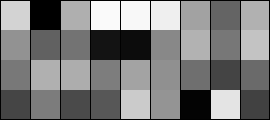
\includegraphics[width=.5\textwidth]{matEx.png}
		\caption{max: 3.97}
	\end{subfigure}
	\caption{The same matrix, in numerical and visual forms}
	\label{fig:matvisex}
\end{figure}\noindent

